\section{Section B}
\label{sec:results}

\subsection{Calculation of maximum bending displacement}
The experimentally generated modulus of elasticity, Eexp, for each of the two materials can be obtained in Table 1.2 of section A. Also the moment of inertia for the beam is $4.5\times 10^{-11}$ which can be obtained in section A.
The maximum bending displacements can be calculated by \begin{large}
$\delta _{Max}=\delta _c=\frac{PL^3}{48EI}$\end{large}. 
\newpage 
The maximum bending displacements of Mild Steel under different loads can be obtained by Equation \ref{E 2.1}.
\begin{Large}
\begin{equation}
	\label{E 2.1}
\left\{ \begin{array}{c}
	\delta _{An\_1}=\frac{P_{50N}L^3}{48E_sI}=\frac{50\times 0.1^3}{48\times 172.6698\times 10^9\times 4.5\times 10^{-11}}=0.1341\times 10^{-3}m\\
	\\
	\delta _{An\_2}=\frac{P_{100N}L^3}{48E_sI}=\frac{100\times 0.1^3}{48\times 172.6698\times 10^9\times 4.5\times 10^{-11}}=0.2681\times 10^{-3}m\\
	\\
	\delta _{An\_3}=\frac{P_{150N}L^3}{48E_sI}=\frac{150\times 0.1^3}{48\times 172.6698\times 10^9\times 4.5\times 10^{-11}}=0.4022\times 10^{-3}m\\
\end{array} \right. 
\\
\end{equation}
\end{Large}
\vspace{-8pt}
The maximum Alumlnilum bending displacementsunder different loads can be obtained by Equation \ref{E 2.2}.
\begin{Large}
\begin{equation}
	\label{E 2.2}
\left\{ \begin{array}{c}
	\delta _{An\_1}=\frac{P_{50N}L^3}{48E_{Al}I}=\frac{50\times 0.1^3}{48\times 63.7500\times 10^9\times 4.5\times 10^{-11}}=0.3631\times 10^{-3}m\\
	\\
	\delta _{An\_2}=\frac{P_{100N}L^3}{48E_{Al}I}=\frac{100\times 0.1^3}{48\times 63.7500\times 10^9\times 4.5\times 10^{-11}}=0.7262\times 10^{-3}m\\
	\\
	\delta _{An\_3}=\frac{P_{150N}L^3}{48E_{Al}I}=\frac{150\times 0.1^3}{48\times 63.7500\times 10^9\times 4.5\times 10^{-11}}=1.0893\times 10^{-3}m\\
\end{array} \right. 
\end{equation}
\end{Large}
\vspace{-10pt}
\subsection{Result of maximum bending displacement}
The maximum bending displacements for Mild Steel and Aluminium at different loads can be obtained from the calculations in section B, part 1, and the results are shown in Table 2.1.
\begin{figure}[htp]
	\centering
	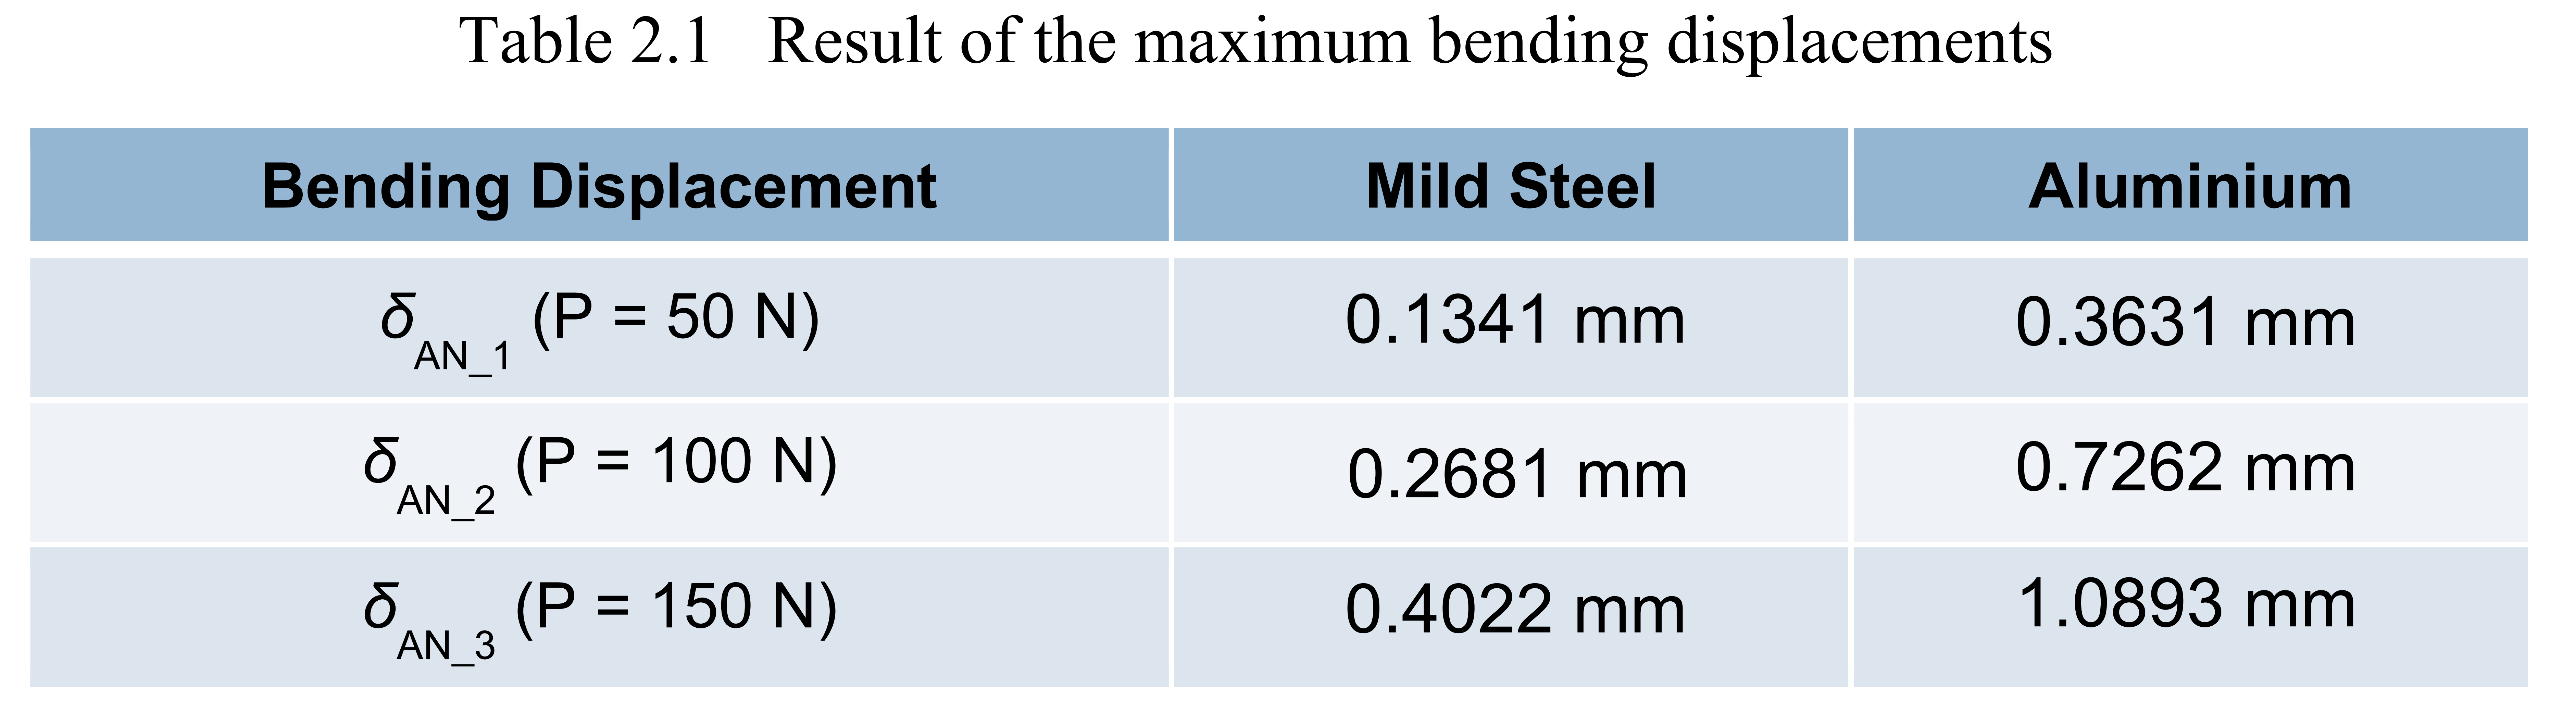
\includegraphics[width=1.0\linewidth]{Results_and_discussion/Figure/RESULT}
    \caption*{}
    \label{T 2.1}
\end{figure}


\FloatBarrier % Now the table doesn't flow over to any other sections